\chapter{VHDL designs in Verilog} \label{ch:VerilogInVhdl}
\chapterquote{Let what comes come. Let what goes go. Find out what remains.}{Ramana Maharshi}

\graphicspath{{Chapters/VhdlWithVerilog/Figures/}}
\lstinputpath{Codes-Verilog/Chapter-VHDL-designs-in-Verilog/VerilogCodes} %path is defined in mypreamble


\section{Introduction}
Since, both VHDL and Verilog are widely used in FPGA designs, therefore it be beneficial to combine both the designs together; rather than transforming the Verilog code to VHDL and vice versa. This chapter presents the use of VHDL design in the Verilog codes. 

\section{VHDL designs in Verilog}

For using VHDL in verilog designs, only proper component instantiation is required as shown in this section. Design of 1 bit comparator in Listing \ref{verilog:comparator1BitVHDL} (which is written using VHDL) is same as the design of Listing \ref{verilog:comparator1Bit}. Design generated by Listing \ref{verilog:comparator1BitVHDL} is shown in Fig. \ref{fig:comparator1BitVHDL}. 

\lstinputlisting[
language = Vhdl,
caption    = {1 bit comparator in Verilog},
label      = {verilog:comparator1BitVHDL}
]{comparator1BitVHDL.vhd}
\begin{figure}[!h]
	\centering
	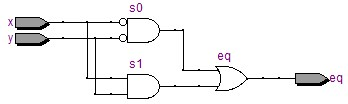
\includegraphics[scale=0.7]{comparator1BitVHDL}
	\caption{1 bit comparator using VHDL}
	\label{fig:comparator1BitVHDL}
\end{figure}

\begin{explanation}[Listing \ref{vhdl:comparator2BitWithVHDL}]
	This listing is exactly same as Listing \ref{verilog:comparator2BitStruct}. To design the 2 bit comparator, two 1 bit comparators are instantiated in line 10 and 11. The final design generated for the two bit comparator is shown Fig. \ref{fig:comparator2BitWithVHDL}. In this way, we can use the VHDL designs in Verilog codes. 
\end{explanation}

\lstinputlisting[
language = Verilog,
caption    = {VHDL design in Verilog},
label      = {vhdl:comparator2BitWithVHDL}
]{comparator2BitWithVHDL.v}
\begin{figure}[!h]
	\centering
	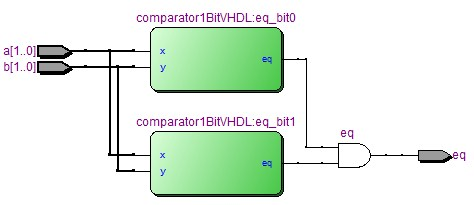
\includegraphics[scale=0.7]{comparator2BitWithVHDL}
	\caption{2 bit comparator using VHDL and Verilog}
	\label{fig:comparator2BitWithVHDL}
\end{figure}

\section{Conclusion}
In this chapter, VHDL files are used in Verilog designs. From the examples shown in this chapter, it is clear that we need not to do anything special to using VHDL files in Verilog designs; only proper port mapping i.e. component instantiation is required. 

